\subsection{Data}\label{subsec:data}
Training a model for human motion analysis requires a great deal of human motion data. There exists two efforts to help in this regard. First of the AMASS data set is an attempt to amass a large quantity of human motion data from motion capture \cite{AMASS:2019}. Secondly the fairmotion library is a library that allows you to take motion from all of the heterogeneous formats currently available, including the AMASS data set, and access all of it through one homogenous interface \cite{gopinath2020fairmotion}. The fairmotion library requires both motion data and skeleton/model data of a human. As such, AMASS was used for the motion data and \cite{MANO:2017} for the skeleton/model data.

Only a subset of the AMASS data set was used. This sped up training by training on less data and it meant not having to stream in training data, as the subset used was small enough to fit into memory.

\subsection{Models}\label{subsec:models}
An autoencoder consists of an encoder and a decoder. The encoder works by taking an input and then encoding it into a smaller space called the latent space. The encoder then decodes the latent value back into something similar to the original input value. Such an operation by itself is pointless, but by doing this we are forcing the model to learn which features of the input are necessary for faithful reconstruction and which features can be discarded. This essentially gives us a compressed version of the input, where each change in the latent space is likely to be clearly visible in the output, similar to principal components analysis~\cite{TODO}.An autoencoder consists of an encoder and a decoder. The encoder works by taking an input and then encoding it into a smaller space called the latent space. The encoder then decodes the latent value back into something similar to the original input value. Such an operation by itself is pointless, but by doing this we are forcing the model to learn which features of the input are necessary for faithful reconstruction and which features can be discarded. This essentially gives us a compressed version of the input, where each change in the latent space is likely to be clearly visible in the output, similar to principal components analysis~\cite{TODO}.


\begin{figure}[h]
\centering
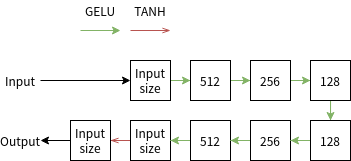
\includegraphics[width=0.5\textwidth]{img/autoencoder}
\caption{Diagram of the model used to implement a simple autoencoder. Each arrow represents a linear layer with either the GELU or tanh activation function applied to its output.}
\label{fig:autoencoder}
\end{figure}

A simple autoencoder using decreasingly smaller/increasingly larger hidden layers for encoding/decoding can be seen in \autoref{fig:autoencoder}. This will be used as a baseline of comparison against the VAE.

Since the above model is bad (non-continuous) we actually want to use a VAE which, TODO: describe VAE and my implementation.

\subsection{Training}\label{subsec:training}
notes on how the training was performed